\documentclass[11pt,a4paper]{article}
\usepackage[a4paper,margin=2.3cm]{geometry}
\usepackage[utf8]{inputenc}
\usepackage[T1]{fontenc}
\IfFileExists{bahasai.ldf}{\usepackage[bahasai]{babel}}{\usepackage[english]{babel}}
\usepackage{booktabs,graphicx,float,amsmath,hyperref,caption,enumitem}
\usepackage[section]{placeins}   % gambar/tabel tidak "kabur" ke bab berikutnya
\captionsetup{font=small}
\hypersetup{hidelinks}
\setlist{nosep}
\graphicspath{{figures/}}
\setlength{\parskip}{4pt}\setlength{\parindent}{0pt}\setlength{\emergencystretch}{3em}
% Dibuat otomatis oleh kode/common/make_tables.py — JANGAN diedit manual.

\newcommand{\TduaCoverageInterval}{0.338}  % t2_experimen.json
\newcommand{\TduaDelta}{-14}  % t2_experimen.json
\newcommand{\TduaKonfigArsitektur}{TCN (1D-CNN dilatasi)}  % t2_terpilih.json
\newcommand{\TduaKonfigBias}{-14.0}  % t2_terpilih.json
\newcommand{\TduaKonfigWindow}{40}  % t2_terpilih.json
\newcommand{\TduaLebarInterval}{10}  % t2_experimen.json
\newcommand{\TduaModelTerbaik}{TCN (1D-CNN dilatasi)}  % t2_experimen.json
\newcommand{\TduaNUnitTest}{300}  % t2_experimen.json
\newcommand{\TduaNUnitTrain}{900}  % t2_experimen.json
\newcommand{\TduaNaNPersen}{2.03}  % t2_experimen.json
\newcommand{\TduaRMSEAsim}{24.57}  % t2_experimen.json
\newcommand{\TduaRMSEGRU}{24.42}  % t2_experimen.json
\newcommand{\TduaRMSELGBM}{20.87}  % t2_experimen.json
\newcommand{\TduaRMSESesudahBias}{22.85}  % t2_experimen.json
\newcommand{\TduaRMSETCN}{20.52}  % t2_experimen.json
\newcommand{\TduaSensorDibuang}{s01, s05, s06, s10, s16, s18, s19}  % t2_experimen.json
\newcommand{\TduaSensorDipakai}{14}  % t2_experimen.json
\newcommand{\TduaSkorAsim}{20,430.2}  % t2_experimen.json
\newcommand{\TduaSkorGRU}{23,278.2}  % t2_experimen.json
\newcommand{\TduaSkorLGBM}{7,072.7}  % t2_experimen.json
\newcommand{\TduaSkorSebelumBias}{6,905.1}  % t2_experimen.json
\newcommand{\TduaSkorSesudahBias}{3,273.4}  % t2_experimen.json
\newcommand{\TduaSkorTCN}{6,905.1}  % t2_experimen.json
\newcommand{\TduaSpike}{22184}  % t2_experimen.json
\newcommand{\TduaUjiMaks}{455}  % t2_experimen.json
\newcommand{\TduaUjiMedian}{162}  % t2_experimen.json
\newcommand{\TduaUjiMedianRUL}{93.8}  % t2_final.json
\newcommand{\TduaUjiMin}{50}  % t2_experimen.json
\newcommand{\TduaUjiServis}{18.7}  % t2_final.json
\newcommand{\TduaUmurMedian}{265}  % t2_experimen.json
\newcommand{\TsatuDomBestFlB}{0.765}  % t1_experimen.json
\newcommand{\TsatuDomFlA}{0.887}  % t1_experimen.json
\newcommand{\TsatuDomFlB}{0.753}  % t1_experimen.json
\newcommand{\TsatuDomTerpilih}{normalisasi per lini}  % t1_experimen.json
\newcommand{\TsatuEnsFl}{0.862}  % t1_final.json
\newcommand{\TsatuEnsFlW}{0.817}  % t1_final.json
\newcommand{\TsatuFlConcat}{0.768}  % t1_experimen.json
\newcommand{\TsatuFlCross}{0.797}  % t1_experimen.json
\newcommand{\TsatuFlImage}{0.579}  % t1_experimen.json
\newcommand{\TsatuFlLate}{0.805}  % t1_experimen.json
\newcommand{\TsatuFlSensor}{0.437}  % t1_experimen.json
\newcommand{\TsatuFusionTerbaik}{late fusion}  % t1_experimen.json
\newcommand{\TsatuKelasGambar}{gores, noda, kontaminasi}  % t1_experimen.json
\newcommand{\TsatuKelasKeduanya}{normal}  % t1_experimen.json
\newcommand{\TsatuKelasKontaminasi}{4.9}  % t1_experimen.json
\newcommand{\TsatuKelasNormal}{49.8}  % t1_experimen.json
\newcommand{\TsatuKelasSensor}{retak, gelembung, las\_dingin}  % t1_experimen.json
\newcommand{\TsatuKonfigDomain}{normalisasi per lini}  % t1_terpilih.json
\newcommand{\TsatuKonfigFusion}{late fusion}  % t1_terpilih.json
\newcommand{\TsatuKonfigNoise}{label smoothing 0.1}  % t1_terpilih.json
\newcommand{\TsatuLiniBTest}{60}  % t1_experimen.json
\newcommand{\TsatuLiniBTrain}{25.1}  % t1_experimen.json
\newcommand{\TsatuMissAsli}{0.814}  % t1_final.json
\newcommand{\TsatuMissHilang}{0.555}  % t1_final.json
\newcommand{\TsatuMissSatu}{0.737}  % t1_final.json
\newcommand{\TsatuNoiseN}{3026}  % t1_experimen.json
\newcommand{\TsatuNoisePersen}{7.88}  % t1_experimen.json
\newcommand{\TsatuNoiseTerpilih}{label smoothing 0.1}  % t1_experimen.json
\newcommand{\TsatuOverfitAkurasi}{100}  % t1_final.json
\newcommand{\TsatuOverfitLoss}{0.0004}  % t1_final.json
\newcommand{\TsatuPikselA}{139.8}  % t1_experimen.json
\newcommand{\TsatuPikselB}{111.7}  % t1_experimen.json
\newcommand{\TsatuSeedMean}{0.858}  % t1_final.json
\newcommand{\TsatuSeedStd}{0.002}  % t1_final.json
\newcommand{\TsatuSeedWMean}{0.811}  % t1_final.json
\newcommand{\TsatuSeedWStd}{0.003}  % t1_final.json
\newcommand{\TsatuSensorHilang}{4.9}  % t1_experimen.json
\newcommand{\TsatuSensorSatuHilang}{8}  % t1_experimen.json
\newcommand{\TsatuUjiNormalPersen}{54.5}  % t1_final.json
\newcommand{\TsatuValBersihPersen}{92.7}  % t1_experimen.json
\newcommand{\TtigaARIDEC}{0.56}  % t3_experimen.json
\newcommand{\TtigaARIGabGambar}{0.9}  % t3_experimen.json
\newcommand{\TtigaARIGabSpek}{0.105}  % t3_experimen.json
\newcommand{\TtigaARIMikroskop}{0}  % t3_experimen.json
\newcommand{\TtigaARIMikroskopFinal}{0}  % t3_final.json
\newcommand{\TtigaClusterTerkecil}{10.2}  % t3_final.json
\newcommand{\TtigaK}{5}  % t3_experimen.json
\newcommand{\TtigaKGambar}{6}  % t3_experimen.json
\newcommand{\TtigaKSpektrum}{5}  % t3_experimen.json
\newcommand{\TtigaKecerahanMdua}{146.1}  % t3_experimen.json
\newcommand{\TtigaKecerahanMsatu}{127.8}  % t3_experimen.json
\newcommand{\TtigaKonfigFusion}{gabungan joint (CLIP)}  % t3_terpilih.json
\newcommand{\TtigaKonfigK}{5}  % t3_terpilih.json
\newcommand{\TtigaKonfigMetode}{GMM (diag)}  % t3_terpilih.json
\newcommand{\TtigaMetode}{GMM (diag)}  % t3_experimen.json
\newcommand{\TtigaNCluster}{5}  % t3_final.json
\newcommand{\TtigaRepTerpilih}{gabungan joint (CLIP)}  % t3_experimen.json
\newcommand{\TtigaSilK}{0.278}  % t3_experimen.json
\newcommand{\TtigaSilRata}{0.278}  % t3_final.json
\newcommand{\TtigaSpikePersen}{0.55}  % t3_experimen.json
\newcommand{\TtigaSpikeSpektrum}{22.5}  % t3_experimen.json
\newcommand{\TtigaStabK}{0.931}  % t3_experimen.json
\newcommand{\TtigaSulitA}{0}  % t3_final.json
\newcommand{\TtigaSulitB}{3}  % t3_final.json


\title{UTS Deep Learning\\\large Klasifikasi Cacat Multimodal, Prediksi Sisa Umur Mesin, dan Clustering Material}
\author{Kelompok 15 \\[4pt] Hadi Nugroho (101032330235) \\ Tarannia Raisha Putri (101032300231) \\ Naufal Alif Abyan (101032300032)}
\date{November 2026}

\begin{document}
\maketitle

\section{Pendahuluan}
Laporan ini menjawab tiga tugas UTS Deep Learning: (1) klasifikasi tujuh jenis cacat produk dari gambar permukaan dan sinyal sensor penekanan,
(2) prediksi sisa umur pakai (RUL) mesin press dari log per siklus, dan (3) pengelompokan sampel material dari citra mikrostruktur dan spektrum komposisi tanpa label.
Model utama setiap tugas adalah jaringan saraf (PyTorch); metode klasik hanya dipakai sebagai baseline atau pembanding. Tiga prinsip dipegang:
\begin{enumerate}
  \item \textbf{Validasi meniru kondisi uji.} Tugas 1 melaporkan F1 per lini dan F1 yang dibobot porsi lini di data uji; Tugas 2 memvalidasi per mesin pada titik potong acak seperti data uji;
        Tugas 3 memeriksa bahwa cluster tidak sekadar memisahkan mikroskop.
  \item \textbf{Tanpa kebocoran.} Statistik normalisasi dihitung dari data latih fold; jendela RUL hanya berisi siklus masa lalu (diuji otomatis).
  \item \textbf{Reproducibility.} Seluruh angka dibaca otomatis dari file hasil di \url{kode/outputs/results/}. Satu perintah menghasilkan ulang semuanya (seed 42):\\
        \texttt{python kode/run\_all.py -{}-task all -{}-mode train}
\end{enumerate}

\section{Tugas 1 -- Klasifikasi Cacat Multimodal}
Data latih: 48.000 unit dengan gambar permukaan $64\times64$ dan sinyal sensor penekanan $3\times128$ (suhu, getaran, arus); data uji 16.000 unit.
Metrik uji adalah macro-F1 tujuh kelas. Validasi memakai 20\% data latih yang dibagi bertingkat menurut kelas $\times$ lini.

\subsection*{(a) Eksplorasi}
Kelas sangat tidak seimbang: \emph{normal} \TsatuKelasNormal\% dan \emph{kontaminasi} hanya \TsatuKelasKontaminasi\% (Tabel~\ref{tab:t1_eda_kelas_missing}).
Gambar contoh tiap kelas dan rata-rata sinyal per kelas ada di Gambar~\ref{fig:t1gambar}--\ref{fig:t1sinyal}. Sensor tidak terekam utuh (ketiga kanal kosong) pada
\TsatuSensorHilang\% unit dan setidaknya satu kanal kosong pada \TsatuSensorSatuHilang\% unit; kekosongan selalu satu kanal penuh, tidak pernah sebagian.
\textbf{Perbedaan train--uji yang besar:} lini B hanya \TsatuLiniBTrain\% data latih tetapi \TsatuLiniBTest\% data uji, dan gambar lini B lebih gelap
(rata-rata piksel \TsatuPikselB{} vs \TsatuPikselA{} pada lini A; Gambar~\ref{fig:t1domain}). Mesin M01--M06 hanya ada di lini A dan M07--M12 di lini B.
Karena itu metrik utama validasi adalah \emph{F1 terbobot uji} $=0{,}4\,\mathrm{F1}_A + 0{,}6\,\mathrm{F1}_B$, yang meniru komposisi data uji.

\begin{figure}[ht]\centering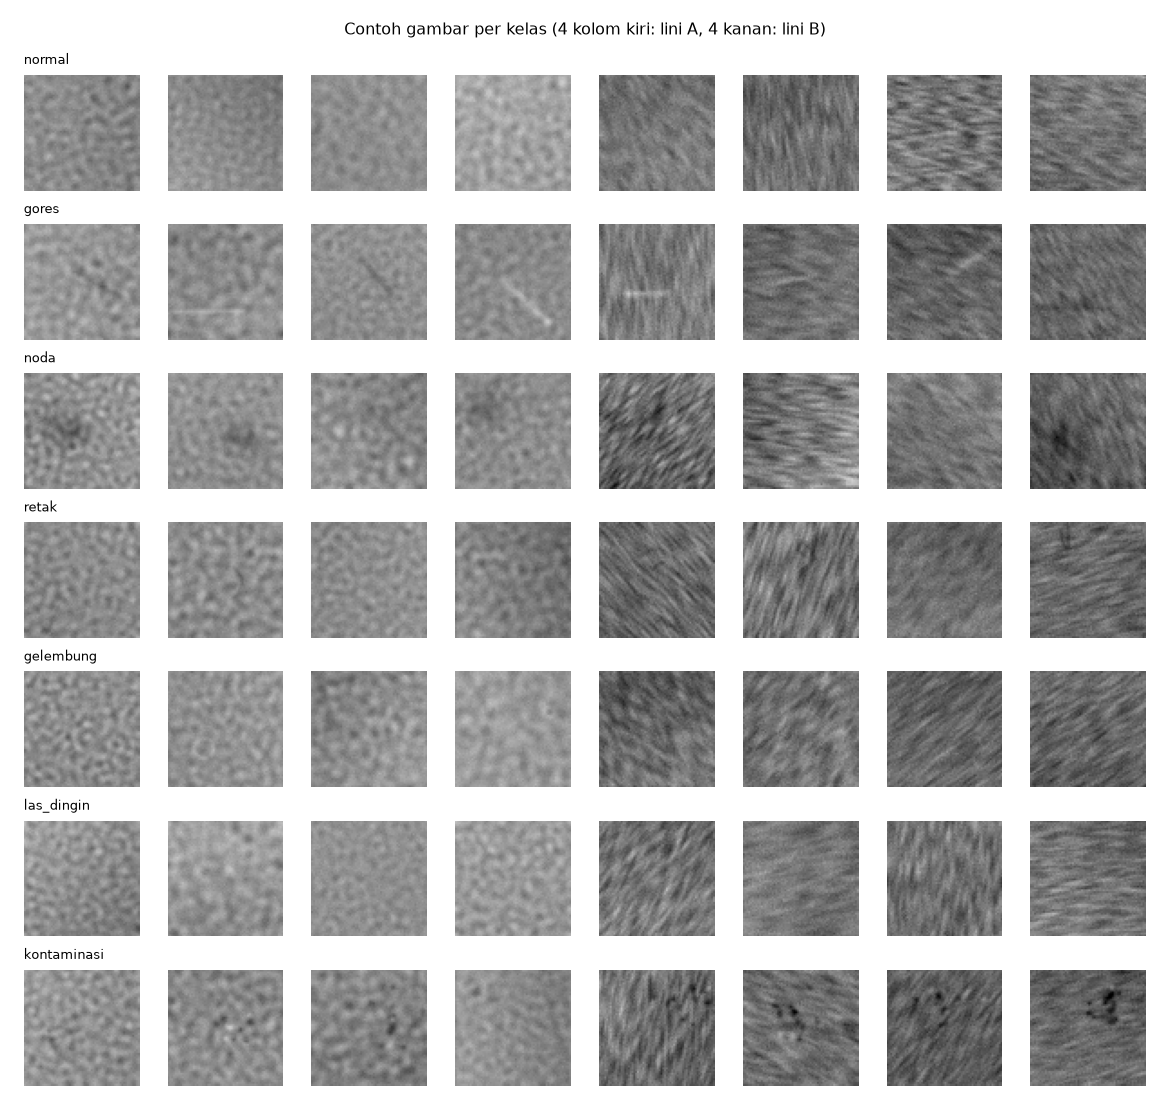
\includegraphics[width=.62\linewidth]{t1_eda_gambar.png}
\caption{Contoh gambar per kelas (kiri lini A, kanan lini B).}\label{fig:t1gambar}\end{figure}
\begin{figure}[ht]\centering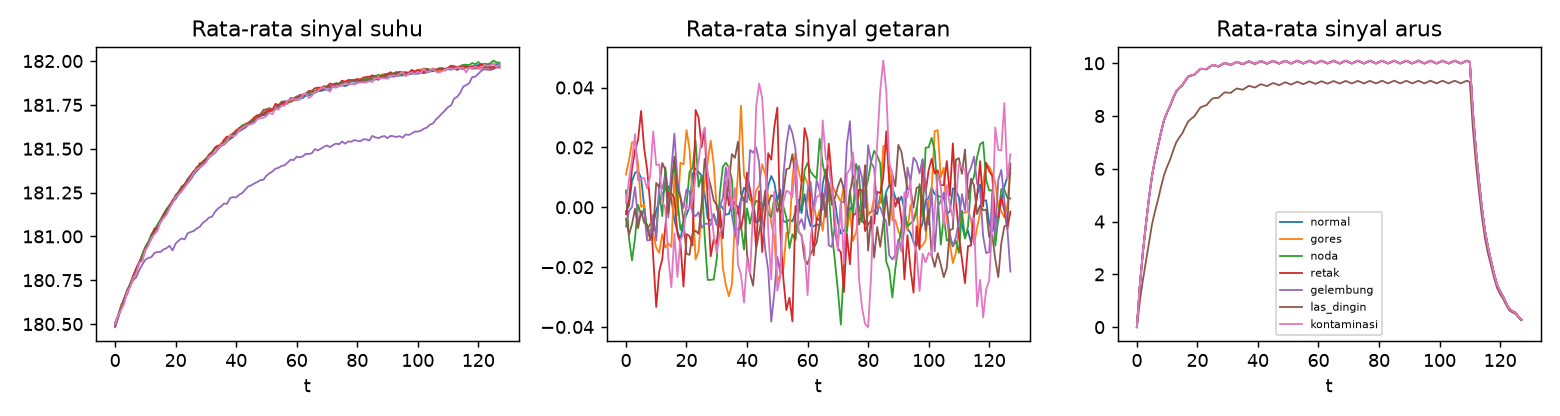
\includegraphics[width=\linewidth]{t1_eda_sinyal.png}
\caption{Rata-rata sinyal tiap kanal per kelas.}\label{fig:t1sinyal}\end{figure}
\begin{figure}[ht]\centering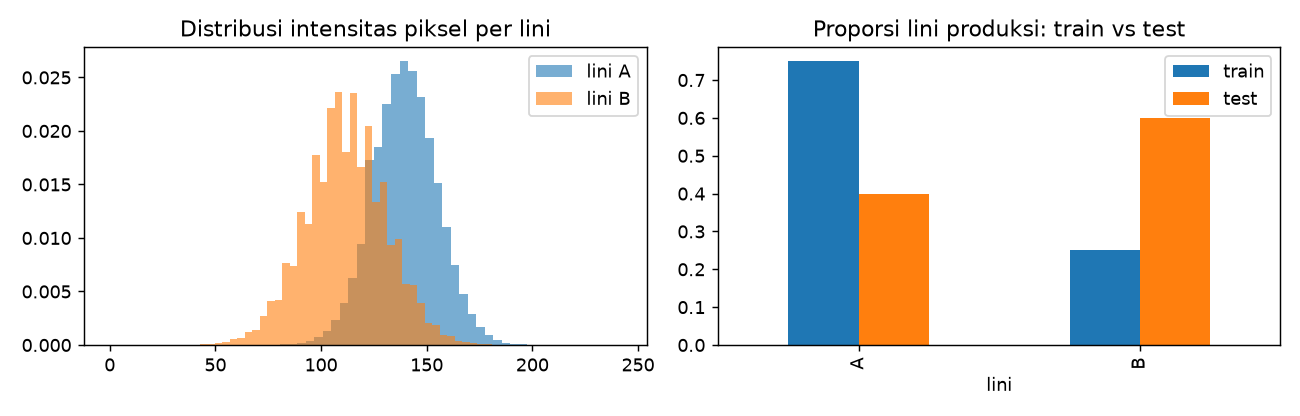
\includegraphics[width=.85\linewidth]{t1_eda_domain.png}
\caption{Intensitas piksel per lini dan proporsi lini di data latih vs uji.}\label{fig:t1domain}\end{figure}
\begin{table}[ht]
\centering\small
\resizebox{\ifdim\width>\linewidth\linewidth\else\width\fi}{!}{%
\begin{tabular}{lrrrrr}
\toprule
kelas & hilang\_suhu\_\% & hilang\_getaran\_\% & hilang\_arus\_\% & hilang\_semua\_\% & porsi\_kelas\_\% \\
\midrule
normal & 5.87 & 5.84 & 5.90 & 4.76 & 49.77 \\
gores & 6.30 & 6.31 & 6.24 & 5.18 & 11.71 \\
noda & 5.93 & 6.10 & 6.14 & 5.17 & 9.94 \\
retak & 6.43 & 6.52 & 6.63 & 5.55 & 7.51 \\
gelembung & 6.18 & 6.03 & 6.01 & 5.10 & 7.15 \\
las\_dingin & 5.78 & 5.69 & 5.57 & 4.70 & 9.01 \\
kontaminasi & 5.30 & 4.96 & 5.18 & 4.16 & 4.91 \\
\bottomrule
\end{tabular}
}
\caption{Distribusi kelas dan persentase kanal sensor yang tidak terekam per kelas.}
\label{tab:t1_eda_kelas_missing}
\end{table}


\subsection*{(b) Arsitektur dan strategi fusion}
\textbf{Encoder gambar:} CNN empat blok (konvolusi $3\times3$--BatchNorm--ReLU dua kali lalu max-pooling) yang menghasilkan peta fitur $256\times4\times4$;
rata-rata globalnya menjadi vektor 256 dimensi dan 16 posisinya menjadi token. \textbf{Encoder sinyal:} 1D-CNN tiga blok; masukannya tiga kanal sinyal
yang dinormalisasi ditambah tiga kanal \emph{mask} (1 = kanal tidak terekam) sehingga model tahu kanal mana yang hilang; keluarannya vektor 128 dimensi dan 16 token.
Tiga strategi fusion dibandingkan dengan seed dan anggaran epoch yang sama (Tabel~\ref{tab:t1_fusion}):
(i) \emph{concat} --- vektor kedua modalitas digabung lalu satu kepala klasifikasi (fusion tingkat fitur);
(ii) \emph{late fusion} --- kepala terpisah per modalitas, logit digabung dengan bobot per kelas yang dipelajari, dan bila seluruh sensor hilang keputusan otomatis dari gambar saja;
(iii) \emph{cross-attention} dua arah antara token gambar dan token sinyal.
Semua model dilatih dengan AdamW, jadwal one-cycle, bobot kelas $\sqrt{1/\text{frekuensi}}$, augmentasi flip/rotasi $90^\circ$, dan \emph{modality dropout}
(sensor dihapus seluruhnya dengan peluang 0,15 dan satu kanal dengan peluang 0,10). F1 terbobot uji: concat \TsatuFlConcat, late \TsatuFlLate, cross-attention \TsatuFlCross;
terpilih \textbf{\TsatuKonfigFusion}.

\begin{table}[ht]
\centering\small
\resizebox{\ifdim\width>\linewidth\linewidth\else\width\fi}{!}{%
\begin{tabular}{lrrrrr}
\toprule
model & f1\_macro & f1\_lini\_A & f1\_lini\_B & f1\_terbobot\_uji & epoch\_terbaik \\
\midrule
concat (early/feature-level) & 0.824 & 0.859 & 0.707 & 0.768 & 11 \\
late fusion & 0.855 & 0.887 & 0.750 & 0.805 & 10 \\
cross-attention & 0.855 & 0.894 & 0.733 & 0.797 & 11 \\
\bottomrule
\end{tabular}
}
\caption{Perbandingan strategi fusion (validasi). F1 terbobot uji = 0.4 F1 lini A + 0.6 F1 lini B.}
\label{tab:t1_fusion}
\end{table}


\subsection*{(c) Nilai tiap modalitas}
Model gambar saja mencapai F1 terbobot \TsatuFlImage{} dan sensor saja \TsatuFlSensor. Per kelas (Tabel~\ref{tab:t1_modalitas}, Gambar~\ref{fig:t1cm}):
kelas yang terutama dikenali dari \textbf{gambar}: \TsatuKelasGambar; dari \textbf{sensor}: \TsatuKelasSensor; yang baru terbaca baik setelah \textbf{fusion}: \TsatuKelasKeduanya.
Hal ini sesuai dengan sifat cacatnya: gores, noda, dan kontaminasi adalah cacat permukaan yang terlihat jelas di citra (Gambar~\ref{fig:t1gambar}), sehingga model sensor saja sama sekali tidak mengenalinya (F1 = 0). Sebaliknya, las dingin tidak tampak di permukaan (F1 gambar saja = 0) tetapi memiliki pola arus dan suhu yang khas saat penekanan (Gambar~\ref{fig:t1sinyal}), sehingga sensor saja sudah mencapai F1 0.93. Retak dan gelembung terbaca dari kedua modalitas, dan fusion menaikkan F1-nya di atas masing-masing modalitas.
\begin{table}[ht]
\centering\small
\resizebox{\ifdim\width>\linewidth\linewidth\else\width\fi}{!}{%
\begin{tabular}{lrrrl}
\toprule
kelas & image-only & sensor-only & fusion (late fusion) & modalitas\_utama \\
\midrule
normal & 0.841 & 0.737 & 0.906 & keduanya (fusion) \\
gores & 0.723 & 0.000 & 0.788 & gambar \\
noda & 0.875 & 0.000 & 0.882 & gambar \\
retak & 0.538 & 0.706 & 0.755 & sensor \\
gelembung & 0.648 & 0.772 & 0.799 & sensor \\
las\_dingin & 0.000 & 0.930 & 0.930 & sensor \\
kontaminasi & 0.913 & 0.000 & 0.924 & gambar \\
\bottomrule
\end{tabular}
}
\caption{F1 per kelas: image-only, sensor-only, dan fusion terpilih (validasi).}
\label{tab:t1_modalitas}
\end{table}

\begin{figure}[ht]\centering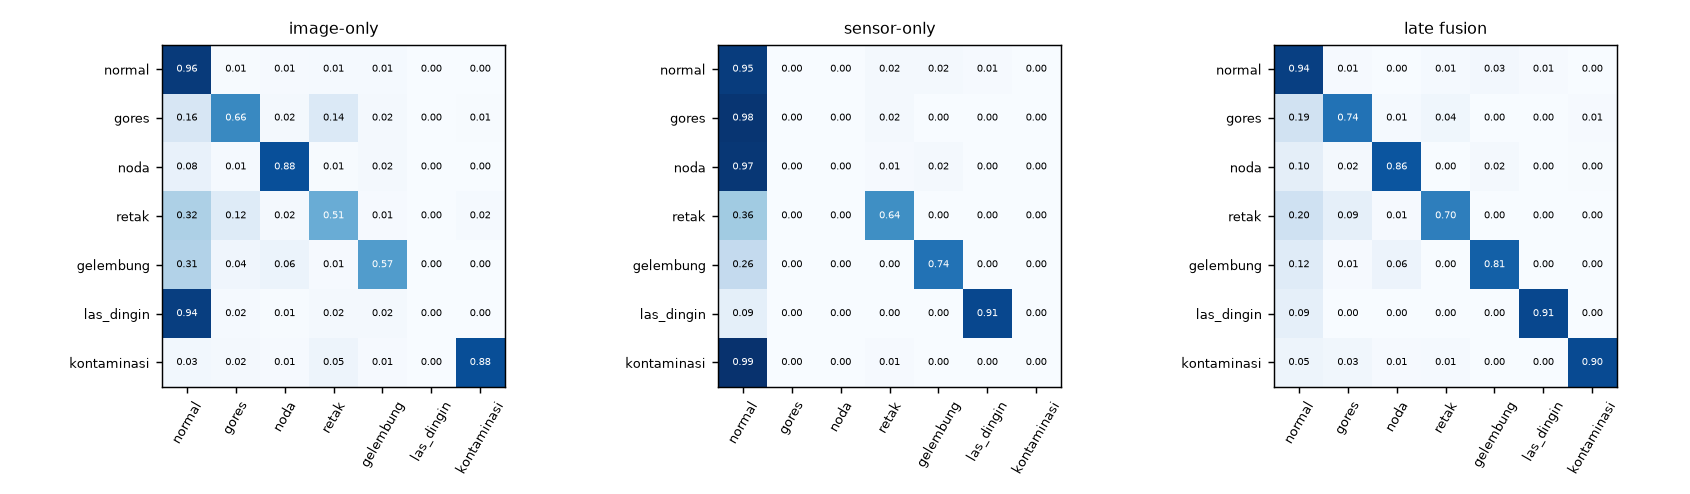
\includegraphics[width=\linewidth]{t1_confusion_modalitas.png}
\caption{Confusion matrix (dinormalisasi per kelas aktual) model gambar saja, sensor saja, dan fusion.}\label{fig:t1cm}\end{figure}

\subsection*{(d) Label tidak sempurna}
Kemungkinan salah label dideteksi dengan \emph{confident learning}: probabilitas \emph{out-of-fold} (3-fold) dari model fusion; ambang per kelas $t_j$ = rata-rata $p_j$ pada
sampel berlabel $j$; sampel dicurigai bila $p(\text{label}) < t_{\text{label}}$ sementara ada kelas lain $j$ dengan $p_j \ge t_j$.
Hasilnya \TsatuNoiseN{} sampel latih (\TsatuNoisePersen\%) dicurigai (Tabel~\ref{tab:t1_label_noise}, contoh di Gambar~\ref{fig:t1noise}).
Dua teknik robust diuji: \emph{label smoothing} 0,1 dan membuang sampel yang dicurigai (Tabel~\ref{tab:t1_robust_noise}). Karena label validasi sendiri bisa salah,
F1 juga dihitung pada validasi tanpa sampel yang dicurigai (\TsatuValBersihPersen\% validasi). Terpilih: \textbf{\TsatuKonfigNoise}.
Sampel yang dicurigai tidak tersebar merata. Menurut kelas, porsi tertinggi ada pada retak (25.4\%), kontaminasi (18.6\%), dan gores (13.8\%), dengan kelas kandidat tersering \emph{gores}; ini wajar karena ketiganya berupa pola garis atau bercak yang mirip secara visual. Menurut lini, porsinya lebih tinggi di lini A (8.8\%) dibanding lini B (5.2\%), dan terkonsentrasi pada mesin M01--M06 (7.9--9.4\%) dibanding M07--M12 (4.5--5.9\%). Sebaliknya, per shift hampir sama (7.7--8.1\%), sehingga kesalahan label kemungkinan berkaitan dengan proses inspeksi di lini/mesin tertentu, bukan dengan shift kerja.
\begin{table}[ht]
\centering\small
\resizebox{\ifdim\width>\linewidth\linewidth\else\width\fi}{!}{%
\begin{tabular}{lrrrl}
\toprule
kelas\_label & n & dicurigai & persen\_dicurigai & kelas\_kandidat\_tersering \\
\midrule
normal & 19110 & 672 & 3.52 & gores \\
gores & 4499 & 622 & 13.83 & normal \\
noda & 3818 & 280 & 7.33 & gores \\
retak & 2885 & 733 & 25.41 & gores \\
gelembung & 2744 & 267 & 9.73 & noda \\
las\_dingin & 3458 & 101 & 2.92 & normal \\
kontaminasi & 1886 & 351 & 18.61 & gores \\
\bottomrule
\end{tabular}
}
\caption{Sampel latih yang dicurigai salah label (confident learning, 3-fold out-of-fold).}
\label{tab:t1_label_noise}
\end{table}

\begin{figure}[ht]\centering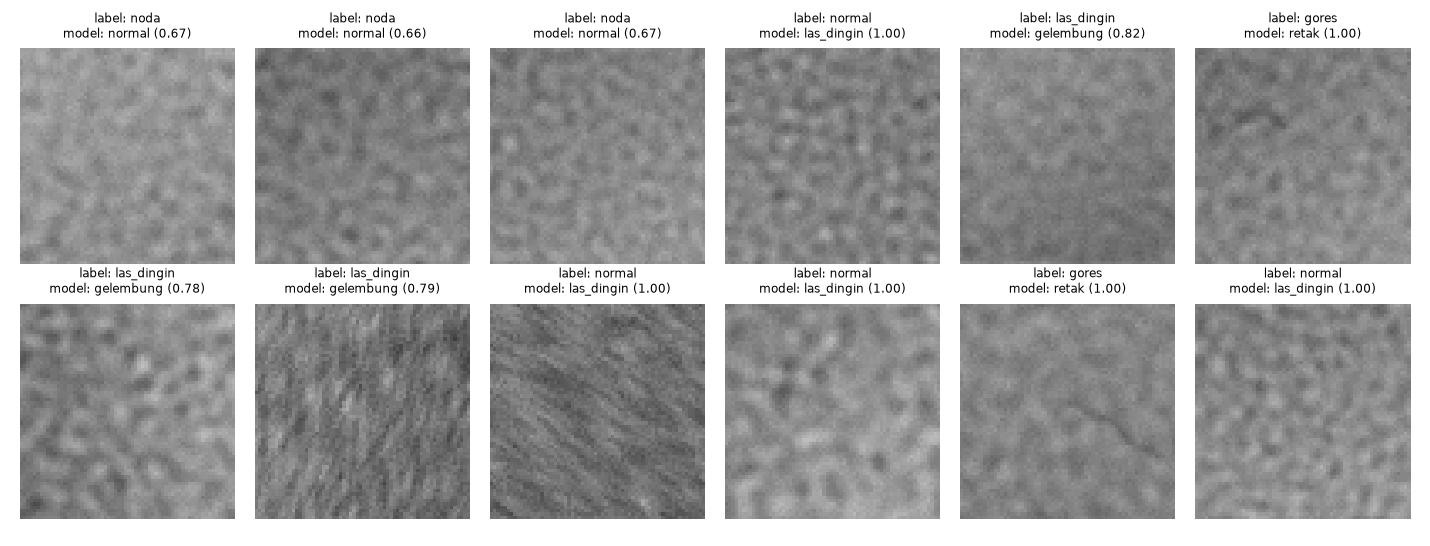
\includegraphics[width=.85\linewidth]{t1_label_noise_contoh.png}
\caption{Contoh sampel yang paling dicurigai salah label: label inspektur vs prediksi model.}\label{fig:t1noise}\end{figure}
\begin{table}[ht]
\centering\small
\resizebox{\ifdim\width>\linewidth\linewidth\else\width\fi}{!}{%
\begin{tabular}{lrrr}
\toprule
teknik & f1\_macro & f1\_terbobot\_uji & f1\_terbobot\_val\_bersih \\
\midrule
baseline (CE + bobot kelas) & 0.855 & 0.805 & 0.884 \\
label smoothing 0.1 & 0.855 & 0.806 & 0.879 \\
buang sampel dicurigai & 0.838 & 0.787 & 0.856 \\
\bottomrule
\end{tabular}
}
\caption{Teknik robust terhadap label noise (validasi penuh dan validasi tanpa sampel yang dicurigai).}
\label{tab:t1_robust_noise}
\end{table}


\subsection*{(e) Domain shift antar lini}
Tanpa penanganan, F1 lini A \TsatuDomFlA{} dan lini B \TsatuDomFlB{} (Tabel~\ref{tab:t1_domain}). Tiga teknik diuji: normalisasi intensitas per lini
(sah karena lini tercantum di metadata uji), augmentasi kecerahan/kontras acak, dan bobot sampel lini B $\times2$. Terpilih \textbf{\TsatuKonfigDomain}
(F1 lini B \TsatuDomBestFlB).

\begin{table}[ht]
\centering\small
\resizebox{\ifdim\width>\linewidth\linewidth\else\width\fi}{!}{%
\begin{tabular}{lrrrr}
\toprule
teknik & f1\_macro & f1\_lini\_A & f1\_lini\_B & f1\_terbobot\_uji \\
\midrule
tanpa penanganan & 0.855 & 0.887 & 0.753 & 0.806 \\
normalisasi per lini & 0.857 & 0.887 & 0.765 & 0.814 \\
augmentasi kecerahan/kontras & 0.853 & 0.887 & 0.745 & 0.802 \\
bobot sampel lini B $\times$2 & 0.848 & 0.876 & 0.758 & 0.806 \\
\bottomrule
\end{tabular}
}
\caption{Domain shift: F1 per lini dan F1 terbobot porsi uji untuk tiap teknik.}
\label{tab:t1_domain}
\end{table}


\subsection*{(f) Sensor yang tidak terekam}
Model final diuji dengan sensor asli, seluruh sensor dihapus, dan satu kanal acak dihapus (Tabel~\ref{tab:t1_missing}): F1 terbobot \TsatuMissAsli, \TsatuMissHilang, dan \TsatuMissSatu.
Berkat kanal mask dan modality dropout, prediksi tetap masuk akal saat sensor hilang; bandingkan dengan model gambar saja (\TsatuFlImage).

\begin{table}[ht]
\centering\small
\resizebox{\ifdim\width>\linewidth\linewidth\else\width\fi}{!}{%
\begin{tabular}{lrrrr}
\toprule
kondisi sensor & f1\_macro & f1\_lini\_A & f1\_lini\_B & f1\_terbobot\_uji \\
\midrule
asli & 0.857 & 0.887 & 0.765 & 0.814 \\
hilang & 0.618 & 0.659 & 0.485 & 0.555 \\
satu\_kanal\_hilang & 0.787 & 0.823 & 0.680 & 0.737 \\
aslinya tidak terekam (n=480) & 0.608 & 0.638 & 0.528 & 0.572 \\
\bottomrule
\end{tabular}
}
\caption{Model final (seed pertama) saat sensor lengkap, seluruhnya hilang, atau satu kanal hilang (validasi).}
\label{tab:t1_missing}
\end{table}


\subsection*{(g) Training: sanity check, learning curve, tiga seed}
Model fusion mampu menghafal satu batch berisi 64 sampel (loss akhir \TsatuOverfitLoss, akurasi \TsatuOverfitAkurasi\%; Gambar~\ref{fig:t1overfit}), tanda bahwa pipeline
data--model--loss benar. Learning curve (Gambar~\ref{fig:t1lc}) dipakai untuk memilih epoch terbaik (early stopping pada F1 terbobot uji).
Tiga seed menghasilkan macro-F1 \TsatuSeedMean{} $\pm$ \TsatuSeedStd{} dan F1 terbobot \TsatuSeedWMean{} $\pm$ \TsatuSeedWStd{} (Tabel~\ref{tab:t1_seed});
ensemble ketiganya (rata-rata softmax) mencapai \TsatuEnsFl{} (terbobot \TsatuEnsFlW) dan dipakai untuk prediksi uji.

\begin{figure}[ht]\centering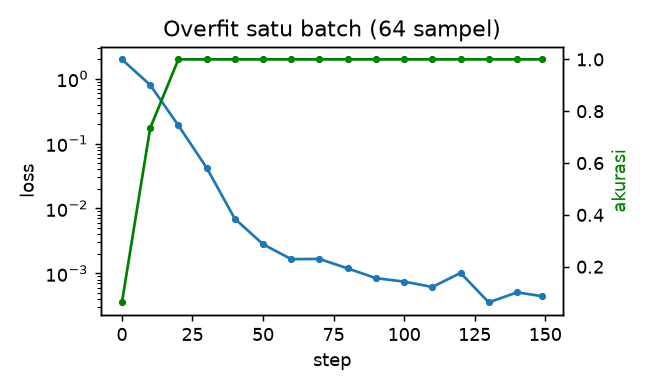
\includegraphics[width=.4\linewidth]{t1_overfit_batch.png}\hspace{1em}
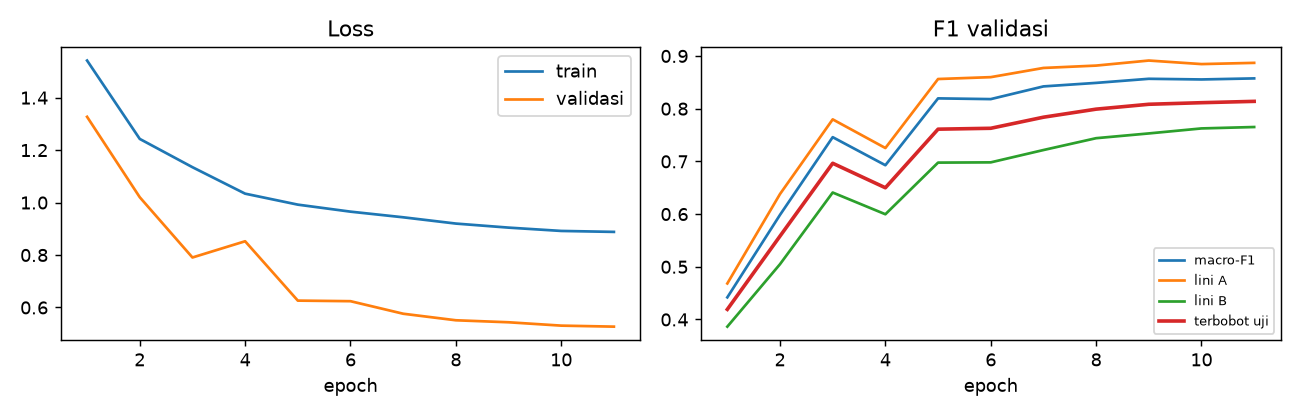
\includegraphics[width=.55\linewidth]{t1_learning_curve.png}
\caption{Kiri: overfit satu batch. Kanan: learning curve model final (seed pertama).}\label{fig:t1overfit}\label{fig:t1lc}\end{figure}
\begin{table}[ht]
\centering\small
\resizebox{\ifdim\width>\linewidth\linewidth\else\width\fi}{!}{%
\begin{tabular}{rrrrrr}
\toprule
seed & f1\_macro & f1\_lini\_A & f1\_lini\_B & f1\_terbobot\_uji & epoch\_terbaik \\
\midrule
42 & 0.857 & 0.887 & 0.765 & 0.814 & 11 \\
43 & 0.860 & 0.894 & 0.756 & 0.811 & 11 \\
44 & 0.857 & 0.890 & 0.753 & 0.808 & 11 \\
\bottomrule
\end{tabular}
}
\caption{Model final dengan 3 seed (validasi).}
\label{tab:t1_seed}
\end{table}


\section{Tugas 2 -- Prediksi Sisa Umur Pakai (RUL)}
Data latih: \TduaNUnitTrain{} mesin dengan riwayat sampai rusak (median umur \TduaUmurMedian{} siklus); data uji \TduaNUnitTest{} mesin yang dipotong pada titik acak
(panjang \TduaUjiMin--\TduaUjiMaks{} siklus, median \TduaUjiMedian). RUL diprediksi di siklus terakhir tiap mesin uji.

\subsection*{(a) Eksplorasi dan preprocessing}
Tiga setelan operasi membentuk enam kondisi diskrit (Tabel~\ref{tab:t2_kondisi}). Bacaan sensor terutama ditentukan oleh kondisi operasi, sehingga tren degradasi
baru terlihat setelah setiap sensor di-z-score \emph{per kondisi} (Gambar~\ref{fig:t2kondisi}); normalisasi global akan menyamarkan tren dengan lompatan antar kondisi.
Statistik normalisasi dihitung hanya dari unit latih pada setiap fold. Bacaan hilang (\TduaNaNPersen\%) diisi dengan nilai sebelumnya dalam unit yang sama
(\emph{forward-fill}, kausal). \emph{Spike} ($|z| > 6$, \TduaSpike{} titik) diganti nilai sebelumnya. Sensor dengan |korelasi Spearman| dengan RUL < 0,05 dibuang
(\TduaSensorDibuang; Tabel~\ref{tab:t2_sensor}), menyisakan \TduaSensorDipakai{} sensor ditambah one-hot kondisi dan nomor siklus.

\begin{figure}[ht]\centering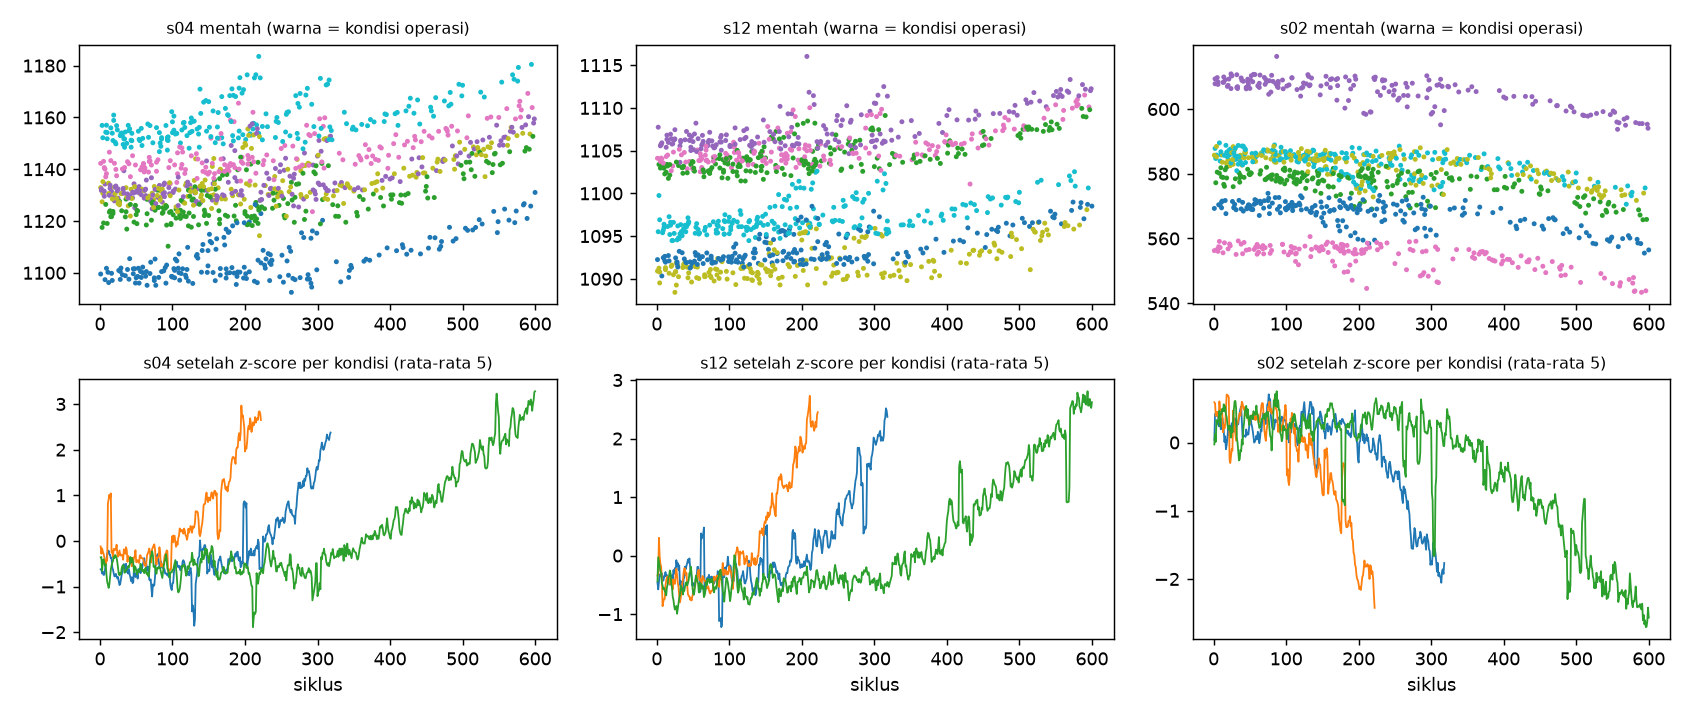
\includegraphics[width=\linewidth]{t2_eda_kondisi.png}
\caption{Atas: sensor mentah (warna = kondisi operasi). Bawah: setelah z-score per kondisi, tren degradasi terlihat.}\label{fig:t2kondisi}\end{figure}
\begin{table}[ht]
\centering\small
\resizebox{\ifdim\width>\linewidth\linewidth\else\width\fi}{!}{%
\begin{tabular}{rrrrr}
\toprule
kondisi & setel\_1 & setel\_2 & setel\_3 & n\_baris \\
\midrule
0 & 20.000 & 0.700 & 100.000 & 42600 \\
1 & 10.000 & 0.250 & 100.000 & 42078 \\
2 & 25.000 & 0.620 & 60.000 & 42211 \\
3 & 42.000 & 0.840 & 100.000 & 42640 \\
4 & 0.000 & -0.000 & 100.000 & 42393 \\
5 & 35.000 & 0.840 & 100.000 & 42252 \\
\bottomrule
\end{tabular}
}
\caption{Enam kondisi operasi hasil clustering setelan (median setelan per kondisi).}
\label{tab:t2_kondisi}
\end{table}

\begin{table}[ht]
\centering\small
\resizebox{\ifdim\width>\linewidth\linewidth\else\width\fi}{!}{%
\begin{tabular}{lrrr}
\toprule
sensor & std\_maks\_per\_kondisi & spearman\_rul & dipakai \\
\midrule
s04 & 8.147 & -0.741 & True \\
s12 & 2.161 & -0.435 & True \\
s15 & 6.544 & -0.430 & True \\
s08 & 4.181 & -0.277 & True \\
s09 & 7.499 & -0.243 & True \\
s18 & 7.922 & -0.001 & False \\
s05 & 2.854 & -0.001 & False \\
s01 & 6.355 & 0.000 & False \\
s16 & 8.082 & 0.001 & False \\
s06 & 4.867 & 0.003 & False \\
s19 & 6.686 & 0.003 & False \\
s10 & 4.538 & 0.003 & False \\
s11 & 13.094 & 0.175 & True \\
s21 & 9.501 & 0.214 & True \\
s20 & 15.333 & 0.235 & True \\
s14 & 7.550 & 0.246 & True \\
s13 & 10.630 & 0.248 & True \\
s17 & 4.181 & 0.253 & True \\
s03 & 9.489 & 0.414 & True \\
s07 & 4.989 & 0.415 & True \\
s02 & 5.481 & 0.425 & True \\
\bottomrule
\end{tabular}
}
\caption{Skor sensor: std maksimum per kondisi dan korelasi Spearman dengan RUL (setelah normalisasi).}
\label{tab:t2_sensor}
\end{table}


\subsection*{(b) Label}
Untuk setiap mesin latih, $\mathrm{RUL}_t = \text{siklus terakhir} - t$, lalu dipotong pada 150 (Gambar~\ref{fig:t2label}): di awal umur mesin, degradasi belum terlihat
sehingga RUL besar tidak dapat dibedakan; pemotongan juga sesuai definisi label uji.

\begin{figure}[ht]\centering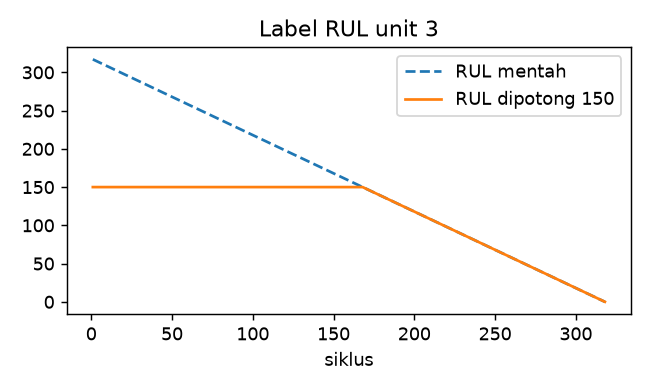
\includegraphics[width=.45\linewidth]{t2_label.png}
\caption{Label RUL mentah dan setelah dipotong 150.}\label{fig:t2label}\end{figure}

\subsection*{(c) Sekuens tanpa kebocoran}
Setiap sampel adalah jendela 40 siklus yang \emph{berakhir} di siklus $t$, dengan target RUL di $t$. Semua mesin disusun dengan padding nol di kiri ditambah kanal mask,
sehingga histori yang lebih pendek dari 40 siklus tetap dapat diproses dan jendela tidak pernah berisi siklus sesudah $t$ atau siklus mesin lain
(diuji otomatis di \texttt{kode/tests/test\_rul\_windows.py}).

\subsection*{(d)--(e) Model dan validasi per mesin}
Dibandingkan GRU dua lapis, TCN (konvolusi kausal berdilatasi 1--8), GRU dengan loss asimetris (kesalahan terlalu optimis diberi bobot 1,6), dan baseline non-DL LightGBM
pada fitur jendela (nilai terakhir, rata-rata 10 siklus, kemiringan 20 siklus). Validasi 3-fold \emph{per mesin} (GroupKFold); setiap mesin validasi dipotong pada tiga
titik acak (panjang $\geq 50$ siklus) seperti data uji, lalu RUL dievaluasi hanya di siklus terakhir yang terlihat --- mengevaluasi semua jendela akan terlalu optimis.
RMSE: GRU \TduaRMSEGRU, TCN \TduaRMSETCN, GRU loss asimetris \TduaRMSEAsim, LightGBM \TduaRMSELGBM; skor asimetris per 300 mesin: \TduaSkorGRU, \TduaSkorTCN, \TduaSkorAsim, \TduaSkorLGBM
(Tabel~\ref{tab:t2_model}--\ref{tab:t2_skor_rentang}). Terpilih \textbf{\TduaKonfigArsitektur}.
Karena skor menghukum prediksi terlambat lebih berat, prediksi digeser $\delta = \TduaKonfigBias$ siklus (dipilih pada prediksi out-of-fold), mengubah skor dari
\TduaSkorSebelumBias{} menjadi \TduaSkorSesudahBias{} dengan RMSE \TduaRMSESesudahBias{} (Gambar~\ref{fig:t2bias}).
Error terbesar ada pada rentang RUL 50--100 (RMSE TCN 29.7, dibanding 12.0 pada RUL 0--25), dan rentang ini juga menyumbang sebagian besar skor asimetris. Pada fase ini degradasi baru mulai sehingga sinyal sensor belum jelas berubah, sedangkan mendekati kerusakan (RUL $<$ 25) tren sensor sudah tegas dan prediksi jauh lebih akurat. Koreksi bias $\delta = -14$ sengaja menaikkan RMSE (20.52 $\to$ 22.85) demi menurunkan skor asimetris hampir separuhnya, karena prediksi yang terlambat jauh lebih mahal daripada yang terlalu dini.
\begin{table}[ht]
\centering\small
\resizebox{\ifdim\width>\linewidth\linewidth\else\width\fi}{!}{%
\begin{tabular}{lrrrrrr}
\toprule
model & rmse & skor\_asimetris\_per\_300\_unit & rmse\_rul\_0\_25 & rmse\_rul\_25\_50 & rmse\_rul\_50\_100 & rmse\_rul\_100\_150 \\
\midrule
TCN (1D-CNN dilatasi) & 20.524 & 6905.118 & 11.988 & 17.677 & 29.691 & 17.000 \\
LightGBM (baseline non-DL) & 20.874 & 7072.671 & 10.927 & 17.727 & 30.636 & 17.175 \\
GRU & 24.416 & 23278.234 & 12.257 & 19.977 & 34.311 & 21.570 \\
GRU + loss asimetris & 24.566 & 20430.217 & 11.035 & 20.502 & 33.458 & 22.566 \\
\bottomrule
\end{tabular}
}
\caption{Perbandingan model (3-fold per mesin, evaluasi di titik potong acak seperti data uji).}
\label{tab:t2_model}
\end{table}

\begin{table}[ht]
\centering\small
\resizebox{\ifdim\width>\linewidth\linewidth\else\width\fi}{!}{%
\begin{tabular}{lrrrr}
\toprule
model & skor\_rul\_0\_25 & skor\_rul\_25\_50 & skor\_rul\_50\_100 & skor\_rul\_100\_150 \\
\midrule
TCN (1D-CNN dilatasi) & 783.576 & 7513.533 & 20794.864 & 1490.349 \\
LightGBM (baseline non-DL) & 689.235 & 7136.239 & 21308.650 & 1677.989 \\
GRU & 865.379 & 59792.506 & 58087.709 & 3257.132 \\
GRU + loss asimetris & 754.139 & 51706.650 & 49658.233 & 3676.140 \\
\bottomrule
\end{tabular}
}
\caption{Skor asimetris per rentang RUL aktual (dinormalisasi per 300 unit).}
\label{tab:t2_skor_rentang}
\end{table}

\begin{figure}[ht]\centering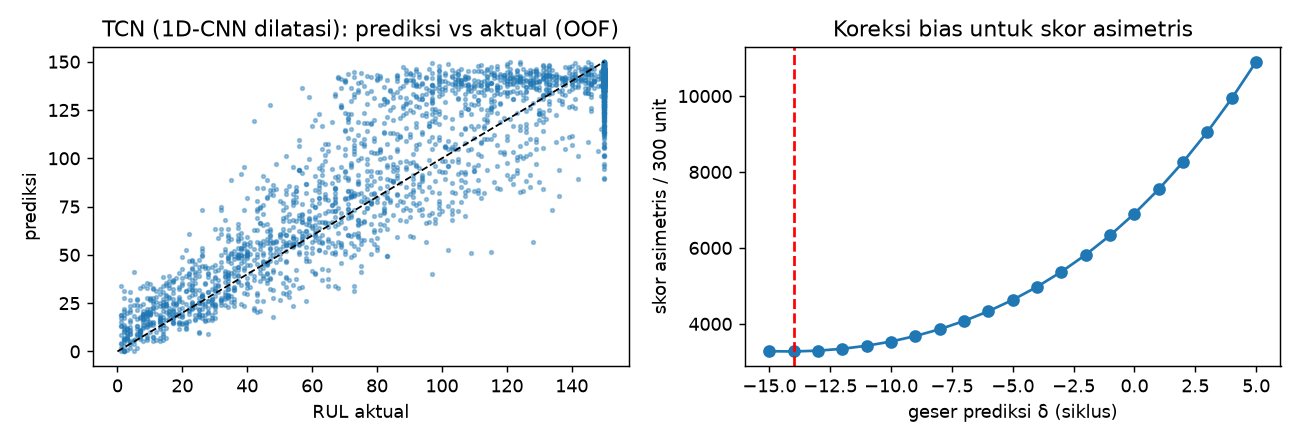
\includegraphics[width=.9\linewidth]{t2_prediksi_bias.png}
\caption{Kiri: prediksi out-of-fold vs aktual. Kanan: pemilihan pergeseran $\delta$ untuk skor asimetris.}\label{fig:t2bias}\end{figure}
\begin{figure}[ht]\centering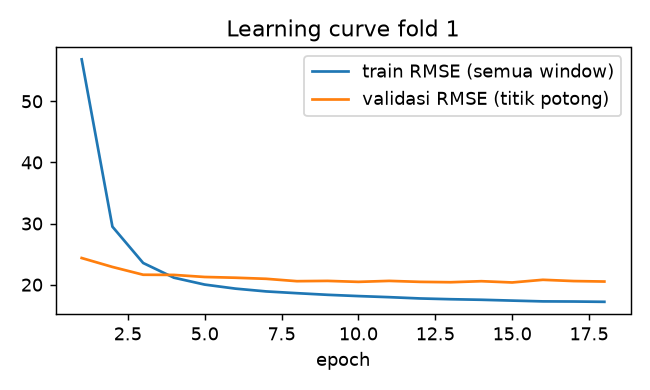
\includegraphics[width=.55\linewidth]{t2_learning_curve.png}
\caption{Learning curve model terpilih pada fold 1: RMSE latih vs RMSE validasi di titik potong.}\label{fig:t2lc}\end{figure}
Gambar~\ref{fig:t2lc} membandingkan RMSE latih (rata-rata semua window) dengan RMSE validasi yang diukur hanya di titik potong seperti data uji. RMSE validasi wajar lebih tinggi karena titik potong lebih sulit diprediksi daripada rata-rata window. Model dilatih dengan jumlah epoch tetap tanpa \emph{early stopping}; sebagai gantinya, risiko overfit diredam dengan dropout, \emph{weight decay}, dan rata-rata tiga seed pada model final. Selisih antara kedua kurva di epoch akhir menunjukkan seberapa besar model mulai menghafal pola data latih.
\subsection*{(f) Ketidakpastian dan kapan servis}
Interval prediksi dibuat dengan MC dropout (30 kali forward dengan dropout aktif pada GRU). Interval 80\% mencakup RUL aktual pada \TduaCoverageInterval{} sampel
validasi dengan lebar median \TduaLebarInterval{} siklus (Gambar~\ref{fig:t2interval}). Kebijakan servis yang diusulkan memakai \emph{batas bawah} interval:
servis bila batas bawah $\leq H$ siklus. Tabel~\ref{tab:t2_kebijakan_servis} menunjukkan trade-off antara mesin hampir rusak yang tertangkap dan servis yang terlalu dini;
dengan $H = 20$, \TduaUjiServis\% mesin uji direkomendasikan diservis.
Kami memilih $H = 30$. Pada validasi, aturan ini menangkap 96.7\% mesin yang benar-benar hampir rusak (RUL $\leq 15$) tanpa satu pun servis yang terlalu dini (RUL $> 80$), dengan 16.0\% mesin diservis; menaikkan $H$ ke 40 hanya menambah tangkapan 3.3 poin tetapi menambah servis. Alasannya, biaya mesin rusak saat produksi (berhenti mendadak dan kerusakan lanjutan) jauh lebih besar daripada biaya satu servis yang agak terlalu awal. Dengan $H = 30$, 23.0\% mesin uji direkomendasikan diservis. Catatan: interval MC dropout terlalu sempit (coverage hanya 0.338 dari target 0.80), sehingga kebijakan ini kami dasarkan pada hasil empiris di validasi, bukan pada nominal 80\%-nya.
\begin{figure}[ht]\centering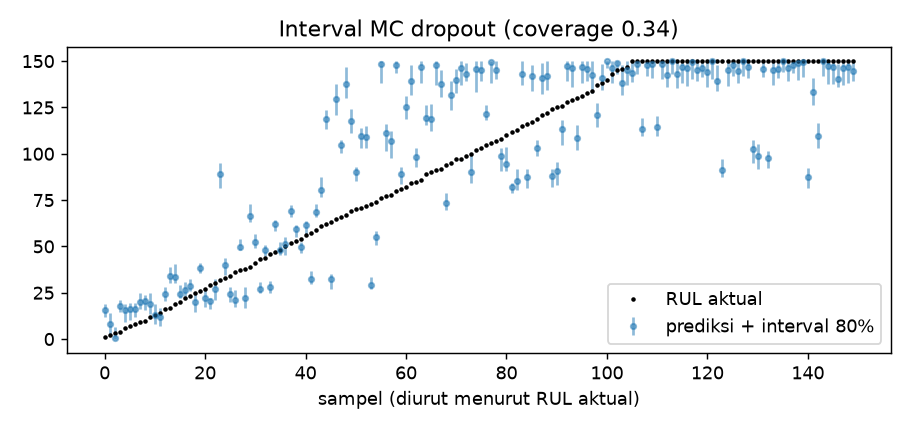
\includegraphics[width=.7\linewidth]{t2_interval.png}
\caption{Prediksi dan interval 80\% MC dropout pada sampel validasi (diurutkan menurut RUL aktual).}\label{fig:t2interval}\end{figure}
\begin{table}[ht]
\centering\small
\resizebox{\ifdim\width>\linewidth\linewidth\else\width\fi}{!}{%
\begin{tabular}{rrrr}
\toprule
H (servis bila batas bawah $\leq$ H) & mesin diservis (\%) & tertangkap, RUL $\leq$ 15 (\%) & terlalu dini, RUL > 80 (\%) \\
\midrule
10 & 5.1 & 51.4 & 0.0 \\
20 & 11.5 & 86.8 & 0.0 \\
30 & 16.0 & 96.7 & 0.0 \\
40 & 20.4 & 100.0 & 0.2 \\
50 & 24.9 & 100.0 & 0.4 \\
\bottomrule
\end{tabular}
}
\caption{Kebijakan servis berbasis batas bawah interval 80\% (MC dropout, GRU, OOF).}
\label{tab:t2_kebijakan_servis}
\end{table}


\textbf{Prediksi uji.} Model terpilih dilatih ulang pada semua mesin latih dengan tiga seed (ensemble), lalu digeser $\delta$ dan dipotong ke $[0,150]$;
median RUL uji \TduaUjiMedianRUL{} siklus. Interval per mesin disimpan di \texttt{kode/outputs/tables/t2\_interval\_uji.csv}.

\section{Tugas 3 -- Clustering Multimodal Material}
Data: 36.000 sampel tanpa label, masing-masing dengan citra mikrostruktur $64\times64$ dan spektrum komposisi 128 titik; dua mikroskop (M1, M2).

\subsection*{(a) Distorsi pada data}
\textbf{Gambar:} orientasi tekstur tersebar merata (rotasi acak), skala bervariasi, dan mikroskop M2 lebih terang (rata-rata \TtigaKecerahanMdua{} vs \TtigaKecerahanMsatu{} pada M1;
Gambar~\ref{fig:t3gambar} dan \ref{fig:t3distorsi}). \textbf{Spektrum:} posisi puncak bergeser beberapa titik, terdapat baseline miring/melengkung, dan \emph{spike} tunggal pada
\TtigaSpikePersen\% titik (\TtigaSpikeSpektrum\% spektrum). Preprocessing spektrum (Gambar~\ref{fig:t3prep}): spike dideteksi sebagai titik yang menyimpang jauh dari rata-rata dua
tetangganya lalu diganti; baseline polinomial derajat 2 di-fit ke ``lantai'' spektrum lalu dikurangkan; terakhir normalisasi SNV. Gambar distandarisasi per mikroskop.

\begin{figure}[ht]\centering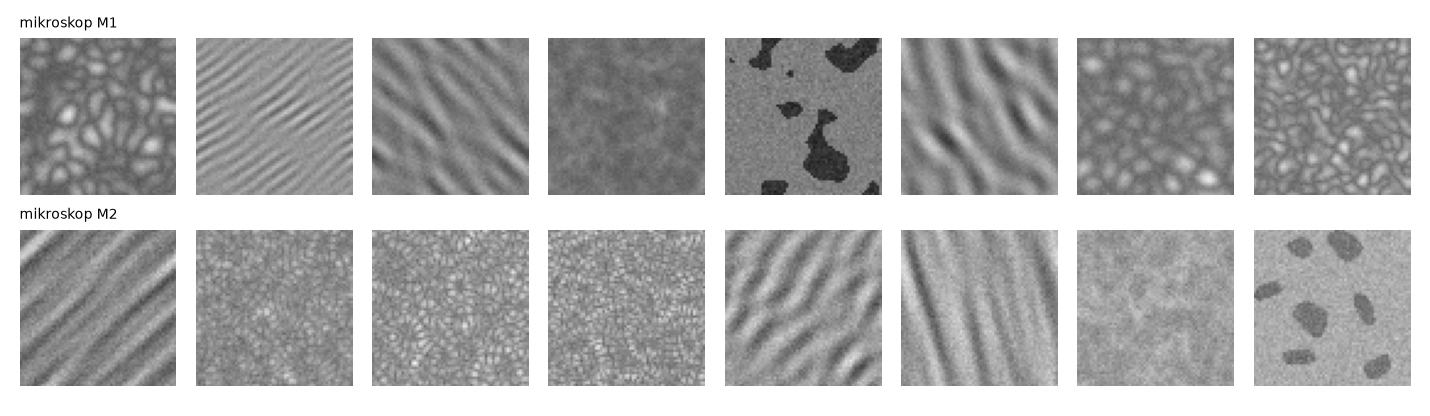
\includegraphics[width=\linewidth]{t3_eda_gambar.png}
\caption{Contoh citra mikrostruktur dari mikroskop M1 (atas) dan M2 (bawah).}\label{fig:t3gambar}\end{figure}
\begin{figure}[ht]\centering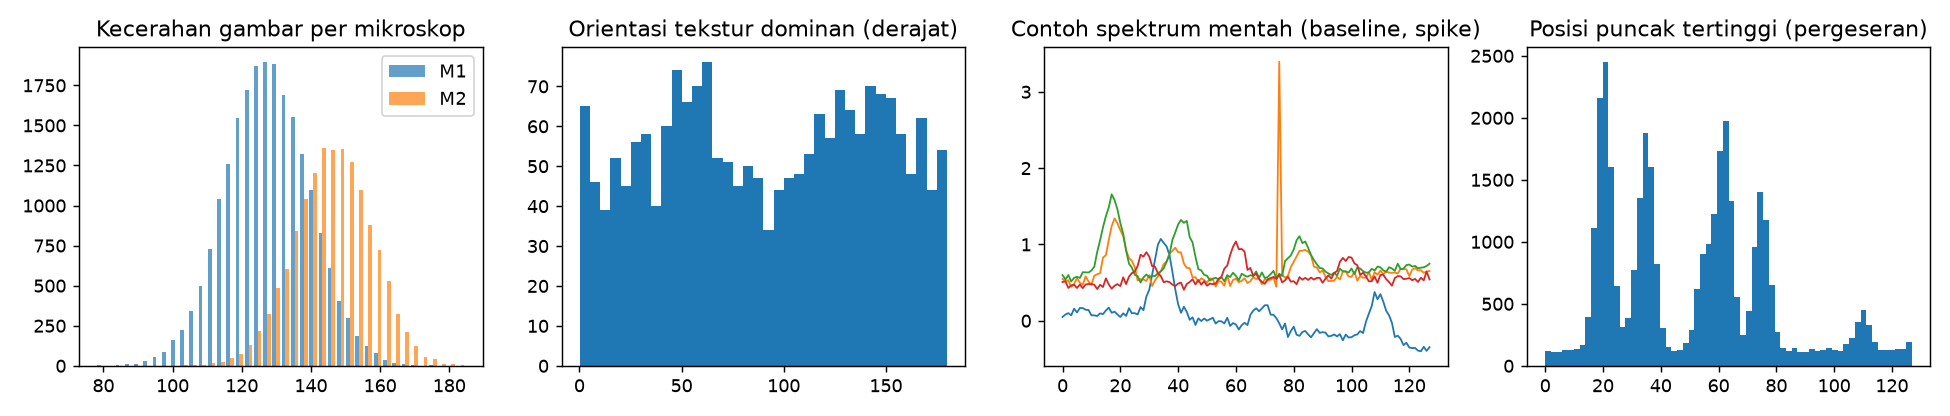
\includegraphics[width=\linewidth]{t3_eda_distorsi.png}
\caption{Kecerahan per mikroskop, orientasi tekstur, contoh spektrum mentah, dan posisi puncak.}\label{fig:t3distorsi}\end{figure}
\begin{figure}[ht]\centering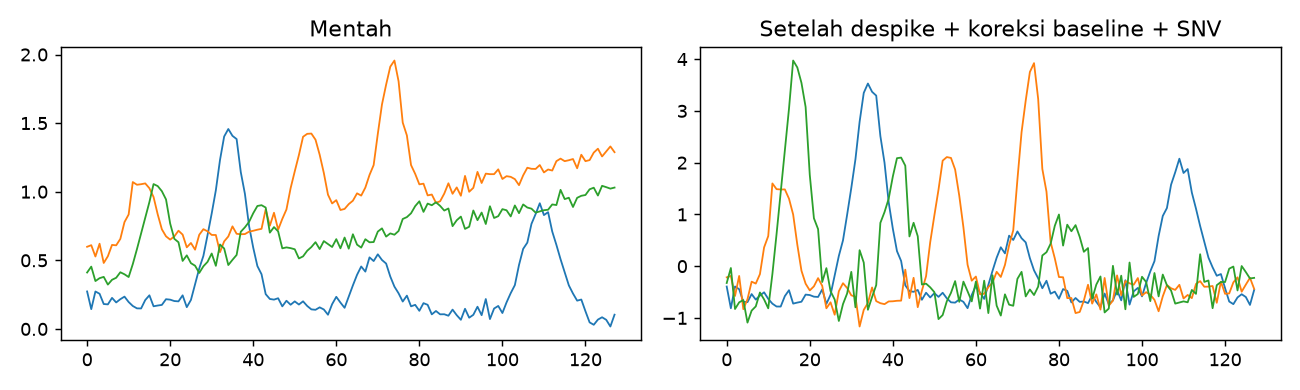
\includegraphics[width=.75\linewidth]{t3_preprocessing_spektrum.png}
\caption{Spektrum sebelum dan sesudah despike, koreksi baseline, dan SNV.}\label{fig:t3prep}\end{figure}

\subsection*{(b) Representasi tanpa label}
Dipakai \emph{SimCLR}: dua augmentasi acak dari sampel yang sama didekatkan dan sampel lain dijauhkan (loss NT-Xent, $\tau=0{,}2$). Augmentasi sengaja meniru
distorsi yang \emph{tidak} boleh memengaruhi tipe material, sehingga representasi menjadi invarian terhadapnya:
\begin{itemize}
  \item gambar: rotasi bebas $0$--$360^\circ$ dan flip (material tidak punya orientasi), skala $0{,}75$--$1{,}25$, kecerahan/kontras (beda mikroskop), blur dan noise;
  \item spektrum: geser $\pm4$ titik (pergeseran puncak), sisa baseline acak kuadratik, spike acak, noise, dan skala intensitas.
\end{itemize}
Encoder gambar adalah CNN yang sama dengan Tugas 1; encoder spektrum 1D-CNN tiga blok. Kurva loss ada di Gambar~\ref{fig:t3loss}.

\subsection*{(c) Dua modalitas}
Dua cara penggabungan dibandingkan: (i) \emph{concat} embedding SimCLR gambar dan spektrum yang dilatih terpisah, (ii) \emph{joint} gaya CLIP --- kedua encoder dilatih
bersama dengan SimCLR per modalitas \emph{ditambah} loss kontrastif lintas-modal (gambar dan spektrum dari sampel yang sama adalah pasangan positif).
PCA piksel+spektrum dilaporkan sebagai pembanding non-DL (Tabel~\ref{tab:t3_representasi}). Representasi gabungan terpilih: \textbf{\TtigaKonfigFusion}.
Dengan gambar saja terpilih $k=\TtigaKGambar$ dan dengan spektrum saja $k=\TtigaKSpektrum$. Kesesuaian cluster gabungan dengan cluster spektrum saja ARI \TtigaARIGabSpek{}
dan dengan gambar saja \TtigaARIGabGambar; crosstab di Gambar~\ref{fig:t3ct} menunjukkan cluster gabungan mana yang \emph{melebur} bila hanya satu modalitas dipakai.
Contoh pasangan yang hanya terpisah oleh gambar adalah cluster 3 dan 4 pada hasil akhir: puncak spektrum keduanya di posisi yang sama (62, Tabel~\ref{tab:t3_per_cluster}), sehingga pembedanya adalah tekstur mikrostruktur. Sebaliknya, pada run ini hampir tidak ada pasangan yang hanya terpisah oleh spektrum: setiap cluster dari gambar saja masuk ke satu cluster gabungan (ARI 0.900), sedangkan kesesuaian dengan cluster spektrum saja rendah (ARI 0.105). Artinya representasi gabungan masih didominasi gambar; ini menjadi keterbatasan sekaligus arah perbaikan, misalnya memberi bobot lebih besar pada loss lintas-modal.
\begin{table}[ht]
\centering\small
\resizebox{\ifdim\width>\linewidth\linewidth\else\width\fi}{!}{%
\begin{tabular}{lrrrr}
\toprule
representasi & k\_terpilih & silhouette & stabilitas\_ARI & ARI\_dengan\_mikroskop \\
\midrule
gambar saja (SimCLR) & 6 & 0.478 & 1.000 & -0.000 \\
spektrum saja (SimCLR) & 5 & 0.243 & 0.978 & -0.001 \\
gabungan concat & 5 & 0.304 & 0.927 & 0.000 \\
gabungan joint (CLIP) & 5 & 0.278 & 0.931 & 0.000 \\
PCA piksel+spektrum (pembanding non-DL) & 5 & 0.208 & 0.968 & 0.002 \\
\bottomrule
\end{tabular}
}
\caption{Representasi: k terpilih (aturan stabilitas $\geq$ 0.90 lalu silhouette tertinggi), kualitas, dan ARI dengan mikroskop.}
\label{tab:t3_representasi}
\end{table}

\begin{figure}[ht]\centering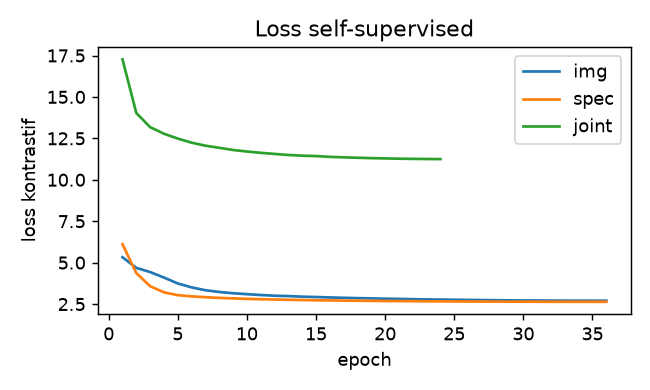
\includegraphics[width=.4\linewidth]{t3_ssl_loss.png}\hspace{1em}
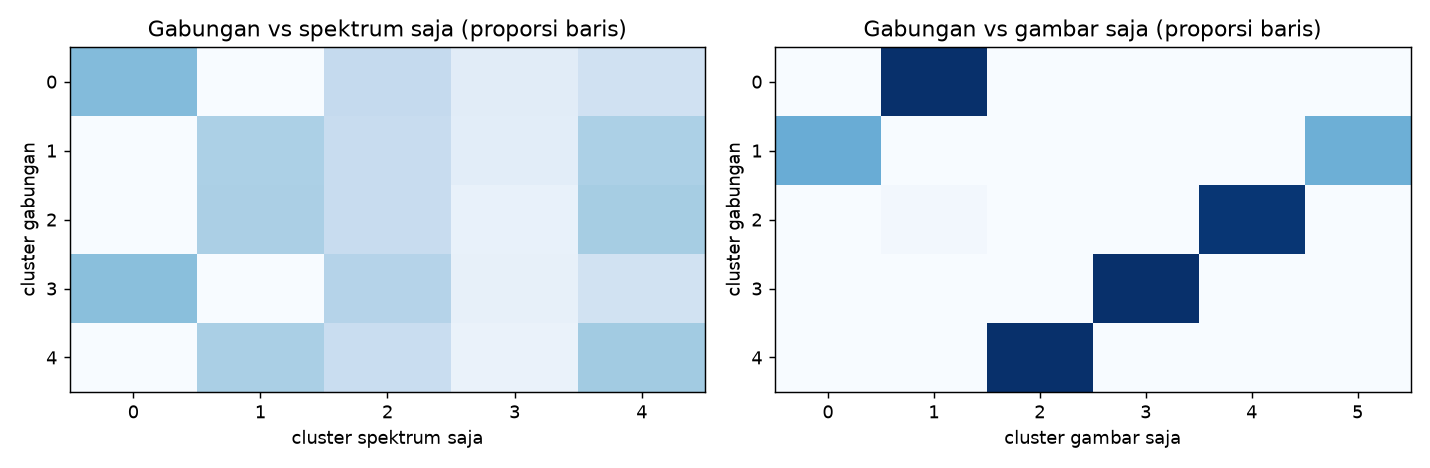
\includegraphics[width=.55\linewidth]{t3_crosstab_modalitas.png}
\caption{Kiri: loss self-supervised. Kanan: cluster gabungan vs cluster satu modalitas (proporsi baris).}\label{fig:t3loss}\label{fig:t3ct}\end{figure}

\subsection*{(d)--(e) Metode dan jumlah cluster}
Pada representasi terpilih, $k = 2,\dots,15$ dinilai dengan silhouette, stabilitas (rata-rata ARI antar 5 run subsampling 80\%), dan BIC GMM (Gambar~\ref{fig:t3k},
Tabel~\ref{tab:t3_kriteria_k}). Aturan yang ditetapkan sebelum melihat hasil: \emph{di antara $k \geq 3$ yang stabil (ARI $\geq 0{,}90$), pilih silhouette tertinggi}.
Terpilih $k = \TtigaK$ (silhouette \TtigaSilK, stabilitas \TtigaStabK). Empat metode dibandingkan pada $k$ tersebut (Tabel~\ref{tab:t3_metode}): K-Means, GMM diagonal,
Agglomerative Ward, dan \emph{DEC} (Deep Embedded Clustering: autoencoder kecil di atas embedding, centroid diinisialisasi K-Means, lalu dioptimasi dengan
KL antara soft assignment Student-$t$ dan distribusi target yang dipertajam). Terpilih \textbf{\TtigaKonfigMetode} (metode paling stabil antar seed).
ARI cluster akhir dengan mikroskop \TtigaARIMikroskopFinal{} $\approx 0$: cluster tidak sekadar memisahkan mikroskop.

\begin{figure}[ht]\centering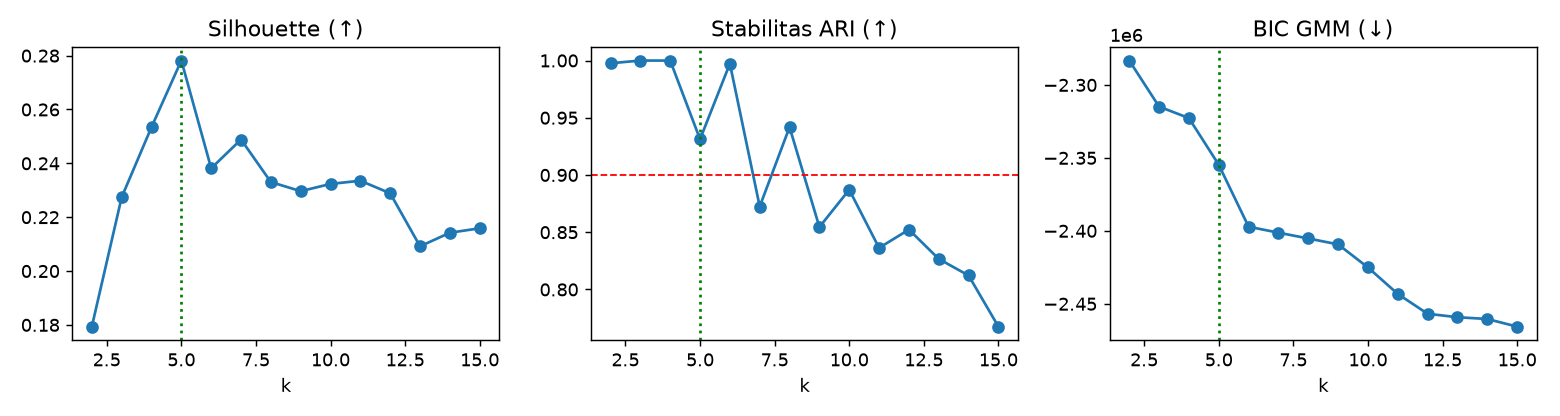
\includegraphics[width=\linewidth]{t3_kriteria_k.png}
\caption{Kriteria jumlah cluster; garis hijau = $k$ terpilih.}\label{fig:t3k}\end{figure}
\begin{table}[ht]
\centering\small
\resizebox{\ifdim\width>\linewidth\linewidth\else\width\fi}{!}{%
\begin{tabular}{rrrrrrr}
\toprule
k & silhouette & davies\_bouldin & bic\_gmm & stabilitas\_ARI & stabilitas\_min & ukuran\_terkecil\_\% \\
\midrule
2 & 0.179 & 2.070 & -2283282.303 & 0.998 & 0.995 & 42.475 \\
3 & 0.227 & 1.837 & -2314852.422 & 1.000 & 1.000 & 24.164 \\
4 & 0.253 & 1.609 & -2322737.164 & 1.000 & 1.000 & 10.156 \\
5 & 0.278 & 1.490 & -2354728.242 & 0.931 & 0.828 & 10.156 \\
6 & 0.238 & 1.484 & -2397181.438 & 0.997 & 0.996 & 10.156 \\
7 & 0.249 & 1.552 & -2401260.713 & 0.872 & 0.770 & 10.156 \\
8 & 0.233 & 1.616 & -2405238.634 & 0.942 & 0.863 & 10.156 \\
9 & 0.230 & 1.541 & -2409291.014 & 0.855 & 0.764 & 7.347 \\
10 & 0.232 & 1.519 & -2425091.265 & 0.887 & 0.825 & 6.667 \\
11 & 0.234 & 1.503 & -2443261.555 & 0.836 & 0.722 & 4.961 \\
12 & 0.229 & 1.492 & -2456844.745 & 0.852 & 0.731 & 4.961 \\
13 & 0.209 & 1.598 & -2459216.140 & 0.827 & 0.694 & 4.936 \\
14 & 0.214 & 1.573 & -2460424.780 & 0.812 & 0.721 & 3.003 \\
15 & 0.216 & 1.593 & -2465670.483 & 0.768 & 0.698 & 4.961 \\
\bottomrule
\end{tabular}
}
\caption{Kriteria jumlah cluster pada representasi terpilih (gabungan joint (CLIP)).}
\label{tab:t3_kriteria_k}
\end{table}

\begin{table}[ht]
\centering\small
\resizebox{\ifdim\width>\linewidth\linewidth\else\width\fi}{!}{%
\begin{tabular}{lrrrrr}
\toprule
metode & silhouette & ARI\_antar\_seed & ARI\_vs\_KMeans & ARI\_dengan\_mikroskop & ukuran\_terkecil\_\% \\
\midrule
K-Means & 0.278 & 0.828 & 1.000 & 0.000 & 10.156 \\
GMM (diag) & 0.278 & 1.000 & 0.992 & 0.000 & 10.156 \\
Agglomerative Ward & 0.278 & 1.000 & 0.999 & 0.000 & 10.156 \\
DEC (deep clustering) & 0.202 & 0.567 & 0.560 & 0.000 & 16.964 \\
\bottomrule
\end{tabular}
}
\caption{Perbandingan metode clustering pada k = 5.}
\label{tab:t3_metode}
\end{table}


\subsection*{(f) Analisis}
t-SNE pada 5.000 sampel (Gambar~\ref{fig:t3tsne}) menunjukkan \TtigaNCluster{} kelompok dan tidak ada pemisahan menurut mikroskop. Ringkasan per cluster
(silhouette, porsi tetangga dari cluster lain, posisi puncak spektrum) ada di Tabel~\ref{tab:t3_per_cluster}; contoh gambar dan spektrum rata-rata di Gambar~\ref{fig:t3contoh}.
Pasangan yang paling sulit dipisah (tetangga terdekat paling sering bercampur) adalah cluster \TtigaSulitA{} dan \TtigaSulitB.
Meski disebut ``paling sulit'', pencampurannya sangat kecil: hanya 0.24\% tetangga terdekat cluster 0 dan 3 berasal dari cluster pasangannya. Puncak spektrum keduanya berbeda (posisi 20 vs 62), sehingga keduanya berdekatan karena tekstur citranya mirip, bukan karena komposisinya sama (Gambar~\ref{fig:t3contoh}). Cluster dengan silhouette terendah justru cluster 2 (0.18), yang menunjukkan materialnya paling bervariasi di dalam kelompoknya.  
\begin{figure}[ht]\centering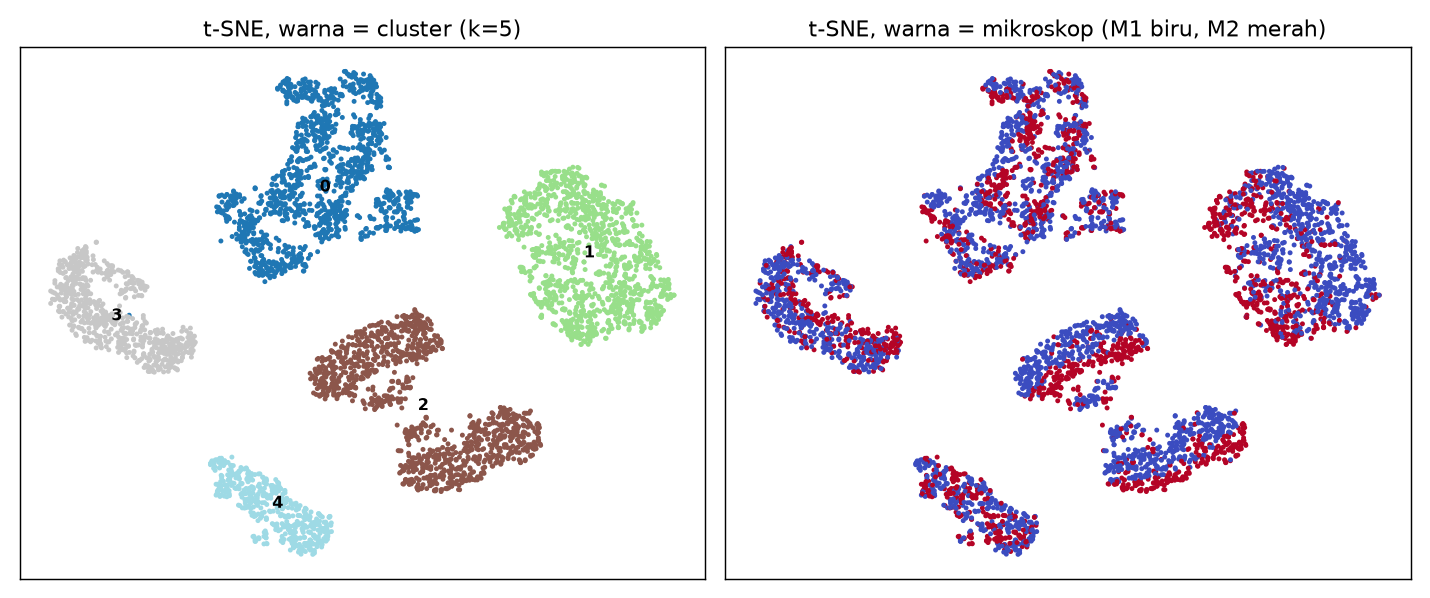
\includegraphics[width=.95\linewidth]{t3_tsne.png}
\caption{t-SNE embedding gabungan: warna menurut cluster (kiri) dan mikroskop (kanan).}\label{fig:t3tsne}\end{figure}
\begin{table}[ht]
\centering\small
\resizebox{\ifdim\width>\linewidth\linewidth\else\width\fi}{!}{%
\begin{tabular}{rrrrrr}
\toprule
cluster & ukuran\_\% & silhouette\_rata2 & porsi\_M2\_\% & tetangga\_beda\_cluster\_\% & posisi\_puncak\_spektrum \\
\midrule
0 & 27.93 & 0.29 & 40.11 & 0.07 & 20 \\
1 & 24.12 & 0.30 & 39.15 & 0.02 & 75 \\
2 & 23.99 & 0.18 & 39.98 & 0.07 & 35 \\
3 & 13.80 & 0.33 & 40.05 & 0.17 & 62 \\
4 & 10.16 & 0.35 & 40.70 & 0.00 & 62 \\
\bottomrule
\end{tabular}
}
\caption{Ringkasan tiap cluster: ukuran, silhouette, porsi mikroskop M2, tetangga terdekat dari cluster lain, posisi puncak spektrum.}
\label{tab:t3_per_cluster}
\end{table}

\begin{figure}[ht]\centering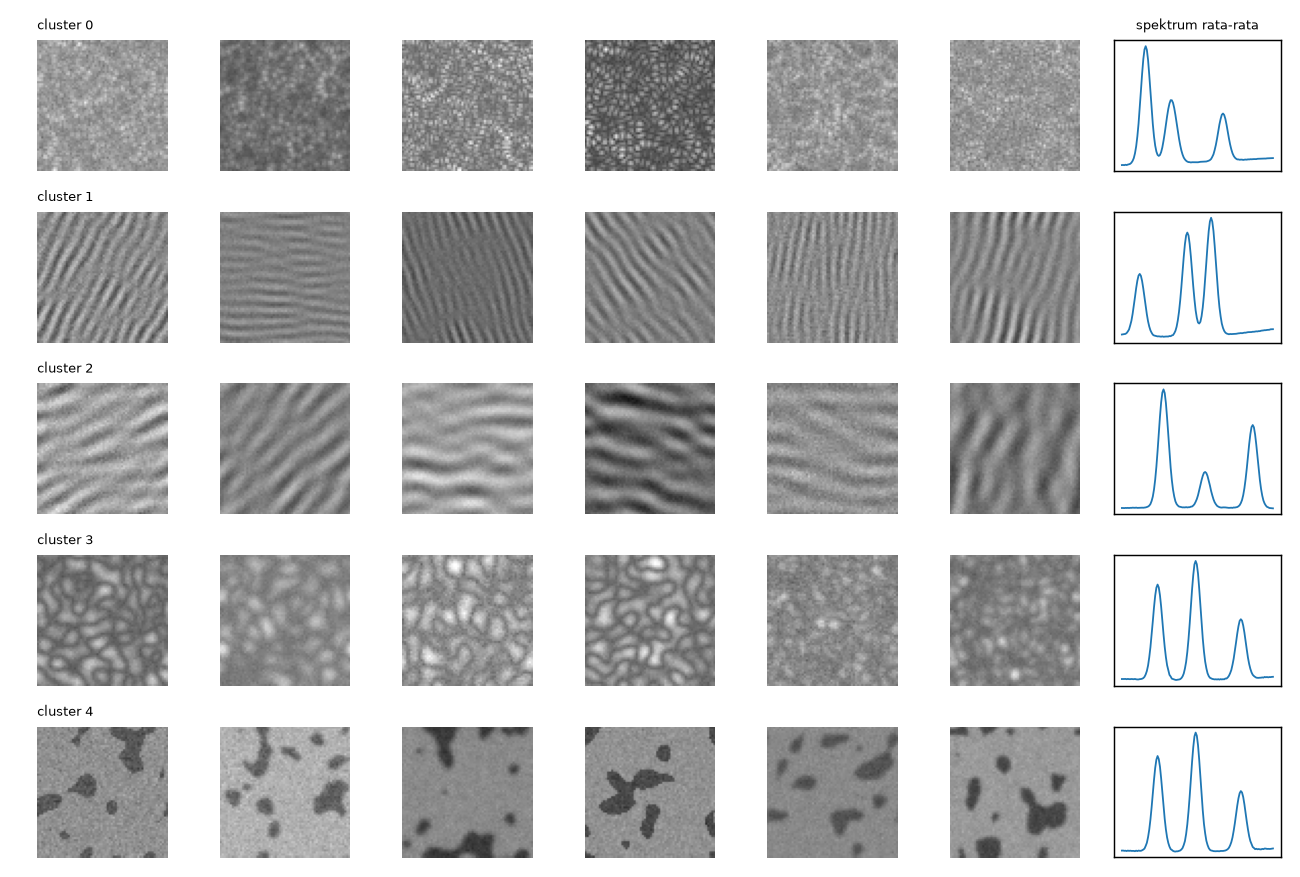
\includegraphics[width=.75\linewidth]{t3_contoh_cluster.png}
\caption{Contoh gambar dan spektrum rata-rata tiap cluster.}\label{fig:t3contoh}\end{figure}


\section{Kesimpulan dan Keterbatasan}
\begin{itemize}
  \item \textbf{Tugas 1.} Perbedaan komposisi lini antara data latih dan uji adalah risiko terbesar; karena itu validasi memakai F1 terbobot porsi lini uji.
        Fusion gambar + sensor dengan kanal mask dan modality dropout menjaga prediksi tetap wajar saat sensor tidak terekam.
        \textit{Keterbatasan:} label validasi sendiri dapat salah, sehingga angka validasi bukan kebenaran mutlak.
  \item \textbf{Tugas 2.} Normalisasi per kondisi operasi dan validasi per mesin pada titik potong acak adalah kunci evaluasi yang jujur. Koreksi bias kecil menurunkan skor
        asimetris karena prediksi terlambat dihukum lebih berat. \textit{Keterbatasan:} interval MC dropout bergantung pada laju dropout dan belum dikalibrasi ulang.
  \item \textbf{Tugas 3.} Augmentasi yang meniru distorsi (rotasi, kecerahan mikroskop, pergeseran puncak, baseline, spike) membuat representasi fokus pada material.
        \textit{Keterbatasan:} jumlah tipe material tidak diketahui; kriteria internal hanya memberi indikasi.
\end{itemize}


\appendix
\section{Lampiran}
\subsection*{A. Reproduksi}
\begin{verbatim}
pip install -r kode/requirements.txt
python -m pytest -q kode/tests
python kode/run_all.py --task all --mode train
python kode/run_all.py --task t1 --mode reproduce
\end{verbatim}
Perintah ketiga menghasilkan semua angka, gambar, tabel, dan tiga file prediksi (GPU T4: ±2--2,5 jam); perintah keempat memuat model tersimpan dan menghitung ulang
angka kunci dalam beberapa menit. Seed 42; versi library dan GPU tercatat di setiap \url{kode/outputs/results/*.json}.

\subsection*{B. Penggunaan AI}
Kode disusun dengan bantuan Claude (Anthropic). Kelompok memverifikasinya dengan tes otomatis (metrik, anti-kebocoran jendela RUL), sanity check overfit satu batch,
membandingkan skema validasi, menjalankan ulang \texttt{-{}-mode reproduce}, dan memeriksa setiap tabel serta gambar. Rincian per anggota ada di \texttt{kontribusi.md}.


\end{document}
